\documentclass[twocolumn]{article}

% Feel free to add more packages
\usepackage{float, amsmath, amssymb, mathtools}
\usepackage{graphicx, caption, color}
\usepackage{tabularx, fullpage}
%\usepackage{kotex}
%\usepackage{multicol}
\setlength{\columnsep}{1cm}
\usepackage{comment, cite, wrapfig}
\usepackage[utf8]{inputenc}
\usepackage[hidelinks]{hyperref}
\usepackage{courier}
%\usepackage{geometry}
\hypersetup{breaklinks=true}
\urlstyle{same}

\newcommand{\red}[1]{{\bf \color{red}#1}}
\newcommand{\blue}[1]{{\bf \color{blue}#1}}
\newcommand{\cut}[1]{}


\begin{document}

\title{Natural Language Interface for Relational Database\\
	\small{Midterm Report}}

%Authors in alphabetical order of last names
\author{Yilin Gao \\
	\small \texttt{yilin.gao@duke.edu} \and 
	Keping Wang \\
	\small \texttt{kw238@duke.edu} \and 
	Chengkang Xu \\
	\small \texttt{cx33@duke.edu} }
	
\date{\today}
\maketitle

%%%================================================================%%%
\section{Introduction}\label{sec:introduction}

Writing SQL queries can be difficult, especially when it involves complex logic. As more and more non-expert users are accessing relational databases, it is very important to simplify their process of writing SQL queries. This project is going to build a Natural Language Interface for relational DataBases (NLIDB), closely following Li and Jagadish (2014)\cite{li2014}. NLIDB will be a tool for everyone to query data easily from relational databases.

Translating natural language into an SQl query isn't an easy job. Not only because of the disambiguity of natural language, but also that users may make mistakes in writing natural language input, such as mis-spelling. We want the users to feel at ease using our interface, not afraid of being mis-interpreted by the NLIDB, even if they cannot remember the exact names of the database column names. So we follow Li and Jagadish (2014)\cite{li2014} to use an interactive interface to let user make choices in several ambiguous phases of the translation.

The main components for translating a natural language to an SQL query are as follows:

\begin{enumerate}
  \item Parse the natural language input into a parse tree using dependency syntax parser.
  \item Map the nodes in the parse tree to SQL keywords, table names, column names, and values. Here users may choose the desired mapping from ranked options.
  \item Adjust the structure of the parse tree to make it follow the structure of an SQL query. Here users may choose the desired structure from ranked options.
  \item Translate the parse tree to an SQL query.
\end{enumerate}

Up until this midterm report, we have completed steps 1 - 2 above. We have built an interactive graphical user interface (GUI), and established connection with a database to experiment with the two steps. Now the user can already choose the desired node mappings from the choices offered by our application. 

Before the final report, we will finish steps 3 - 4 and tune the model with some hand-written natural language and SQL query pairs. 

%%%================================================================%%%
\section{Related Work}

Early day NLIDB systems were usually based on small scale database, which requires a small set of supported queries. Their parsing mechanism could only support ad-hoc methods and rules. Thus, early work would produce ambiguity if the database is scalable and natural language queries are "open-domain". Moreover, without the help of machine learning, early NLIDB systems cannot update their parsing methods as they accumulate more data.\cite{QATutorial}

Our approach involves machine learning in parsing the natural language input into a parse tree. Then we adjust the structure of the parse tree to obey with the SQL syntax. Our approach can handle natural language input with more complicated structures than the simple key-word matching method. 

NLIDB here is a concrete application of the natural language QA systems.\cite{QATutorial} Currently, the mainstream approach for QA is the semantic parsing of questions. It can map natural language questions to logic forms or structured queries, and produce accurate answers when the query is complete and clear. However, the accuracy of answers will decrease if the input language is ambiguous, or if the logic relationship of the query is complicated. Due to our lack of training data, our NLIDB system cannot adopt the popular RNN (LSTM) for a direct and efficient translation. Still we are trying to allow more input ambiguity and structural complexity by letting the users choose the mappings and structures interactively.

%%%================================================================%%%
\section{Problem Definition}

For this NLIDB, we have to first develop a GUI, and then design the \texttt{ParseTree} class. Then we need to develop parse tree node mapper, parse tree structure adjuster, and SQL query translator.

There are three main problems that we face. The first one is the use of data structure in \texttt{ParseTree}. The second is what algorithms to use for each phase of the translation. The last problem is to specify the rules for different phases, such as what word should be mapped to the ``SELECT'' key word, and what rules should a legal parse tree follow before being translated to an SQL query.

%%%================================================================%%%
\section{Algorithms}

In the natural language parsing phase, we use the feature based pos-tagger\cite{toutanova2003feature} and the neural network dependency parser\cite{chen2014fast} from the Stanford NLP package.

In the node mapping phase, other than mapping words with hard coded rules, we compare words with table and column names in the database, which requires a word similarity score. The similarity score is the maximum of two subscores. The first is lexical similarity (similarity in spelling), which is Jaccord coefficient here. The second is semantic similarity, for which we use WUP similarity\cite{wu1994verbs}. To compute WUP similarity, we have to do a breadth-first-search to find the lowest common ancestor of two words in the WordNet. The calculation of word similarity will be explained in detail in the next section.

More algorithms will be needed for parse tree adjustment and SQL query generation in the future.

%%%================================================================%%%
\section{System Design}

\begin{figure*}[ht]
  \centering
  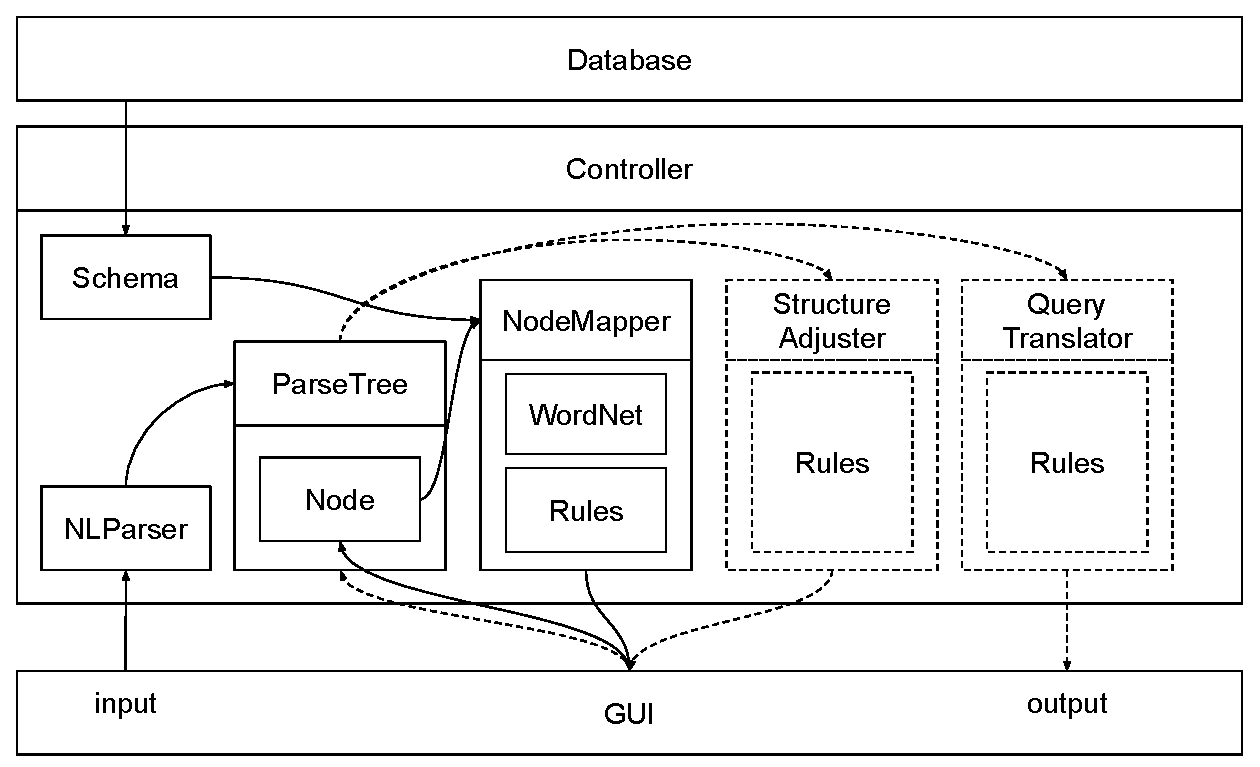
\includegraphics[width=0.8\linewidth]{figures/nlidb_system_diagram.pdf}
  \caption{System Diagram}
\end{figure*}

Our current system is implemented in Java, using maven as the project management tool. The source code are divided into three parts: model, control, and view. The model part takes care of how to realize major functions of the natural language database interface, like parsing natural language, mapping nodes, adjusting node tree structure, and translating the tree into SQL query. The controller wraps many models as attribute variables, and it takes charge of the interaction between database and the view (GUI). And the view part uses JavaFX to design a GUI.

Figure 1 is a diagram of our system. The boxes with solid frame lines are the ones we've already written, and the boxes with dashed frame lines are to be completed in the future. 

Below we’ll introduce the design ideas on two steps that we’ve completed: parsing natural language into a parse tree, and mapping the nodes of the parse tree to SQL components.

\subsection{Natural Language Parser}
We write the NLParser class to parse natural language from the user input in GUI to a dependency parse tree. The NLParser is just a wrapper of the Standford NLP pos-tagger and dependency syntax parser. A natural language sentence is first tagged with part-of-speech labels, and then parsed with dependency parser to a ParseTree.

A ParseTree consists of an array of Nodes. Each Node has information about the natural language word and its corresponding SQL component. A Node also contains parent and children links pointing to other Nodes in the ParseTree.

\subsection{Node Mapper}
Then we map each of the Node into an SQL component. We iterate over the tree and map each Node according to a certain Node Type in Figure 2, according to predefined rules. There are 7 node types in total, and 5 of them, SN, ON, FN, QN, and LN have hard-coded mapping rules. For example, map word “return” or “Return” to an “SN” node with value “SELECT”. A word will first be searched against these five Node Types. If there is no match, the search will go on to the remaining two types, NN and VN.

\begin{figure}[ht]
  \centering
  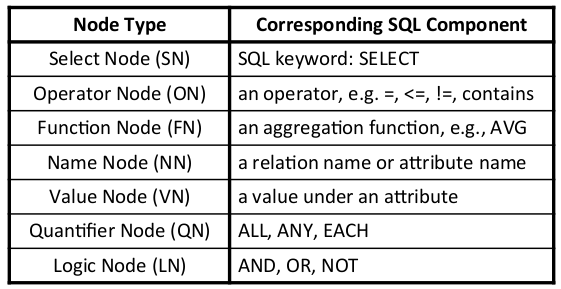
\includegraphics[width=0.9\linewidth]{figures/nodes_mapping_rules.png}
  \caption[caption for nodes mapping rules]{Nodes Mapping Rules\protect\footnotemark}
\end{figure}
\footnotetext{Taken from \cite{li2014}.}

The remaining two types, Name Node and Value Node, are decided by searching over the database for matching names or values. The matching of word to names or values are decided by the word similarity score of two words.The word similarity score here is the maximum of semantic similarity and lexical similarity.

Semantic similarity is the WUP similarity\cite{wu1994verbs} function using WordNet. WordNet is a net of synonym sets (synsets) connected with semantic and lexical pointers. Two most important semantic pointers are hypernym and hyponym, which connect the synsets to the tree that we are interested here, as Figure 3. In Figure 3, the WUP similarity between $C1$ and $C2$ is:

$$ Sim_{WUP} = \frac{2*N3}{N1+N2+2*N3} $$

\begin{figure}[ht]
  \centering
  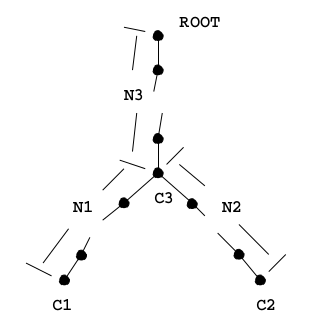
\includegraphics[width=0.7\linewidth]{figures/wordnet_tree.png}
  \caption[caption for wordnet tree]{WUP word similarity.\protect\footnotemark }
\end{figure}
\footnotetext{Taken from \cite{wu1994verbs}.}

One thing to note about WordNet is that each word can be in multiple synsets, and each synset can have multiple parents, so we use breadth-first-search to find the lowest of all possible common parents of two words.


For lexical similarity between two words, we use the Jaccard coefficient:

$$ J(A, B) = \frac{|A \cap B|}{|A \cup B|}$$

where $A$ and $B$ are the set of characters of the two words respectively. The Jaccard coefficient may not be as good for measuring the lexical similarity of two words (as edit distance), but it is currently still used because it is a measure in range (0,1), which makes it easily compared with the WUP semantic similarity.

To search over the database, we first visit the database, retrieve its schema, and store the Schema Graph as an attribute variable in the Controller class, so that each node mapping task don’t have to go through the slow database query. The Schema contains the table names, the column names of each column, and some sample distinct values of each column, such that they can be searched over to map Name Node or Value Node.

Once we have the word similarity scores of one word to names and values in database, we rank different mapping choices by their similarity score, and return the highest several choices to the GUI for the user to choose. Here we add another node type for the user to choose from, that is “UNKNOWN”, which means that node doesn’t correspond to any meaningful SQL component. These meaningless nodes will be removed in later steps.

Figure 4 is an example of a parse tree with nodes mapped to SQL components. The left part is a parse tree, and the right part is the mappings of all its nodes.

\begin{figure}[ht]
  \centering
  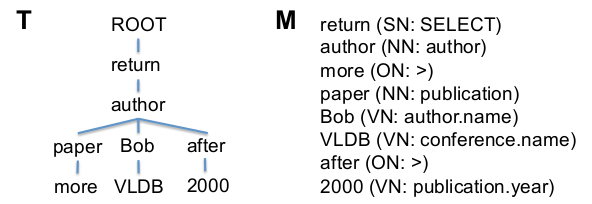
\includegraphics[width=0.9\linewidth]{figures/nodes_mapping_example.png}
  \caption[caption for nodes mapping example]{Node Mapping Example.\protect\footnotemark }
\end{figure}
\footnotetext{Taken from \cite{li2014}.}

\subsection{Node Mapper}
The main idea of inserting implicit node into parse tree is to make sure that two nodes which are being mapped have corresponding schema in database. Assuming invalid nodes are removed from the tree properly, there shoud be a tree with at most three branches. The leftmost tree should contain select node (SN) and name node (NN). If a name node in the left tree does not have ancestor, then it is the core node of the left tree. If the type of core node in left tree is different from right tree, the real core node in right tree is deemed hidden, i.e. implicit. The implicit core node may cause unresonable comparision between two variables of different types due to the change of semantic meaning. An example of implicit node: return all author who wrote more than 100 paper. In our previous process of the parse tree, the right subtree should contain only the number 100, which is a value node (VN). In order to make the tree semantically meaningful, nodes in left subtree are copied over to the right subtree.

After inserting name node based on the core node comparision, next step is to check the constrain for both core node. For example: if left core node has constrain of year greater than 2007 and area of "Database" , right core node should also have the same constrain. If right node does not conform to this constrain, then constrains nodes should be copied from the left subtree to right subtree. 

Our implementation of processing the implicit nodes insertion starts from the root of the tree. It checks if any nodes below select Node (SN) is missing in the middle treel. If there is, copy it over to the middle tree. Then repeat the same procedure to the middle tree and rightmost subtree. After the name node is copied over, it starts from the middle tree to check if there is any constrain missing in the rightmost tree. If there is, copy those over

%%%================================================================%%%
\section{Experiments}
The JavaFX application runs on JVM, and we’ve tested it on an Ubuntu 16.04 machine. We are using JDBC to connect to the PostgreSQL database of dblp, which we used in homework 1.

Our program has already finished part of final target. 

\begin{figure}[ht]
  \centering
  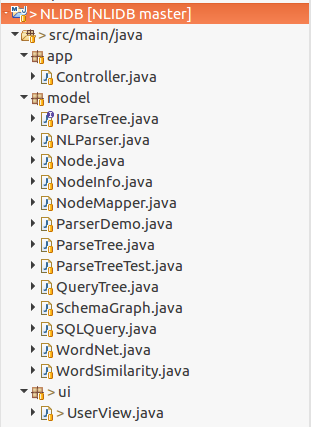
\includegraphics[width=0.8\linewidth]{figures/program_structure.png}
  \caption{Program Structure}
\end{figure}
  
Figure 5 is a detailed structure on programs that we have already finished or at least conceived.

We have programmed a GUI in \texttt{UserView.java} and a connection between database and GUI in \texttt{Controller.java}. To realize natural language query, our first step in implementing the translation process is to parse the natural language into SQL keywords using a predefined natural language parser called Stanford NLP. The parsing process is written in \texttt{NLParser.java} and \texttt{ParserTree.java}. After we get the parser tree, we map each tree node (word in initial natural language input) to certain component of SQL and database. The mapping is written in \texttt{NodeMapper.java}.

\begin{figure*}[ht]
  \centering
  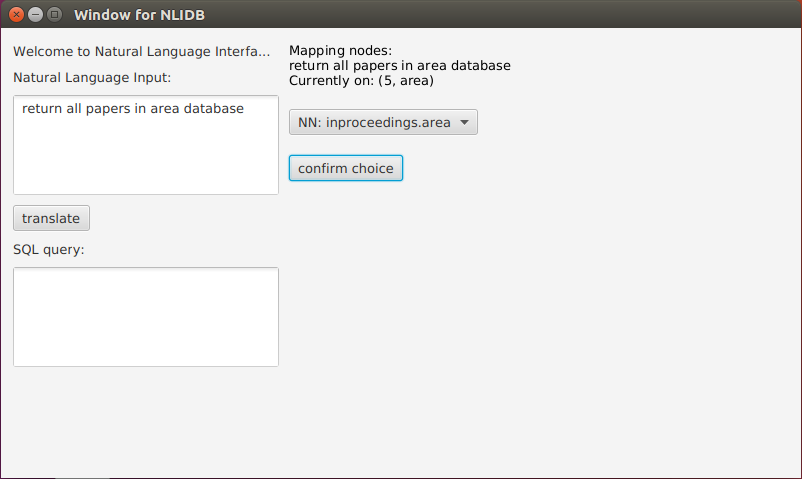
\includegraphics[width=0.7\linewidth]{figures/gui_nodes_mapping.png}
  \caption{GUI during Node Mapping}
\end{figure*}

Figure 6 is a screenshot of our application during the nodes mapping stage. The upper left part is where the user input comes. The bottom left part is supposed to be the translated SQL query (which hasn’t been completed). The upper left part shows the current information on nodes mapping. The choice box showing “NN: inproceedings.title” contains a drop down list of node types and values for the user to choose from. Once the user confirms the choice by pressing the “confirm choice” button, the app will go on to map the next word. The mapping choices will only be shown to the user if the word doesn’t match with the five predefined node types.

As for the node mapper, currently we’ve only defined very limited number of explicit rules for nodes mapping. There are only a few predefined keywords, such as return, equals, all, etc (thus limited SQL query functions as well). We plan to tune the app after we’ve completed writing the whole process of translation. The nodes mapping for name nodes and value nodes doesn’t work perfectly well, maybe in the future we will try some more sensible measures of word similarity. But it is ok for now, since the users can almost always find the right name node or value node from the multiple choices. 

As for basic GUI functions, we may need to design a much fancier GUI as the last step of our program.

%%%================================================================%%%
\section{Contributions of Project Members}

\begin{itemize}
\item {\bf Yilin Gao:} GUI implementation, controller design, report writing.
\item {\bf Keping Wang:} database connection, schema retrieval, Stanford NLP parser usage, parse tree design, word similarity score, report writing.
\item {\bf Chengkang Xu:} node mapping, meaningless nodes removal, inserting implicit nodes, report writing.
\end{itemize}


\Urlmuskip=0mu plus 1mu\relax
\bibliographystyle{abbrv}
\bibliography{nlidb}

\end{document}
